\documentclass[UTF8,12pt,oneside]{ctexart}
\usepackage{graphicx}
\usepackage{xeCJK}
\usepackage{indentfirst}
\usepackage{titletoc}
\usepackage{fancyhdr}
\usepackage{fontspec}

%\setmainfont{Times New Roman}
%\pagestyle{plain} % 此处为fancy时有页眉
%\title{\textbf{\fontsize{42}{84}{反雷杂志 \\[15] Anti-Lei Magazine}}}
%\author{\Large \kaishu 雷氏力学吧、太差太差吧内部资料 \\[8] \Large \kaishu 《反雷杂志》编辑部 \\[8] \Large \kaishu 责任编辑:Mono6 \\[8] \Large \kaishu 封面设计:拆家大主教}
%\date{\huge 2021年5月第2期 \\ (总第2期)}

\begin{document}

如图,一只猴子固定在地面上。将质量为$m$的子弹以$L_0$的运动力射入猴子的脑袋,子弹在猴子脑袋中所受阻力与子弹速度的关系为$F(v)=-iv$($i$为常数)。假设子弹始终做直线运动,且猴脑足够大。

\begin{center}
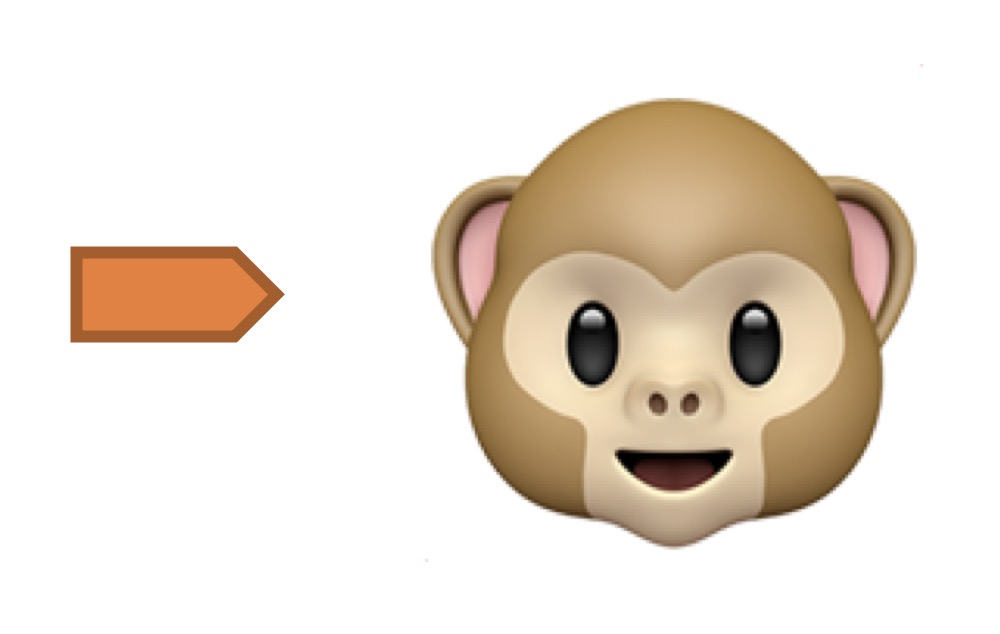
\includegraphics[scale=0.15]{fig1.jpg}
\end{center}

(1) 若子弹在猴脑中做猛减速运动,求常数 $i$ 的取值范围;

(2) 若子弹在猴脑中不做猛减速运动,求子弹在猴脑中第 $t$ 秒的运动力 $L(t)$ 的表达式;

(3) 求子弹在猴脑中经历的总路程 $s$。


\end{document}